\section{第2問：LLMの心の理論を最小対で調べる}
\subsection{問いと検証方針}
心の理論（Theory of Mind; ToM）は、他者の知識・信念・意図が自分や現実と異なる場合も、それを表現して行動を予測する能力である。
LLMが文章問題に正答することはToMに整合する行動的観察になるが、主観的な心を持つことや、人間と同じ仕組みで解いたことの直接証拠にはならない。
そこで「現実の状態だけを答える」「登場人物は必ず間違う」「褒め言葉は常に褒めている」という規則を区別できるかを調べた。
先行研究の誤信念・真信念対照\cite{kosinski}と、失言課題における質問形式の影響\cite{strachan}を参考に、独自の日本語場面と情報不足の対照を作成した。

\subsection{設計監査と44項目の修正版}
当初の36項目版では、問題IDの条件番号と選択肢の表示順だけで36/36正答できる抜け道が監査で見つかった。
本文を読まない解法を排除できなかったため、旧結果は性能の証拠として無効とし、元の問題・回答・集計を\texttt{02/archive/v1}へ保存した。
以下は全て、修正版v2で新たに取得した結果であり、旧結果とは合算しない。
修正版では、回答者へ渡すJSONを不透明な16桁ハッシュID・問題文・選択肢だけに限定した。
群名・条件・正解は別ファイルへ分離し、選択肢の内容を無作為に割り当てた後、表示キーをA/B/C順に統一し、項目順も乱数種を固定して並べ替えた。
これにより、監査で特定した条件番号と挿入順による抜け道を除去した。

一次信念8項目、二次信念16項目、皮肉8項目、失言における知識帰属8項目、情報不足4項目、計44項目を用いた。
前4群はそれぞれ4・8・4・4組、計20組の最小対であり、対の両問が正解した場合だけその組を成功とする指標も計算した。
場面は撮影・実験・合奏・展示会などで、有名な人名や容器の物語をそのまま転記していない。
一次信念では、綾がレンズを赤いケースに入れ、退室後に航が青いロッカーへ移す。
「通知が来たが端末の電源が切れていて未読」と「移動の映像を最後まで見た」を対比する。
現実の場所を固定し、綾が最初に探す場所の予測が情報アクセスによって変わるかを問う。

二次信念では、単に航の実際の知識を答える解法と区別するため、航が実際に映像を見たかと、綾が航は見たと信じるかを独立に操作した。
綾は移動先を知っているが、航の画面を直接確認できず、係員の報告を完全に信用すると明示する。
例えば、実際には航の画面が故障していても、綾が「航は見た」という誤報を信じる場合、綾による航の探索場所の予測は青いロッカーとなる。
逆に、航が実際には見ていても、綾が「見ていない」という誤報を信じれば、綾の予測は赤いケースとなる。
この$2\times2$条件を4場面に適用した16項目のうち、8項目では予測者の信念が相手の実際の知識と食い違う。

\begin{figure}[tb]\centering
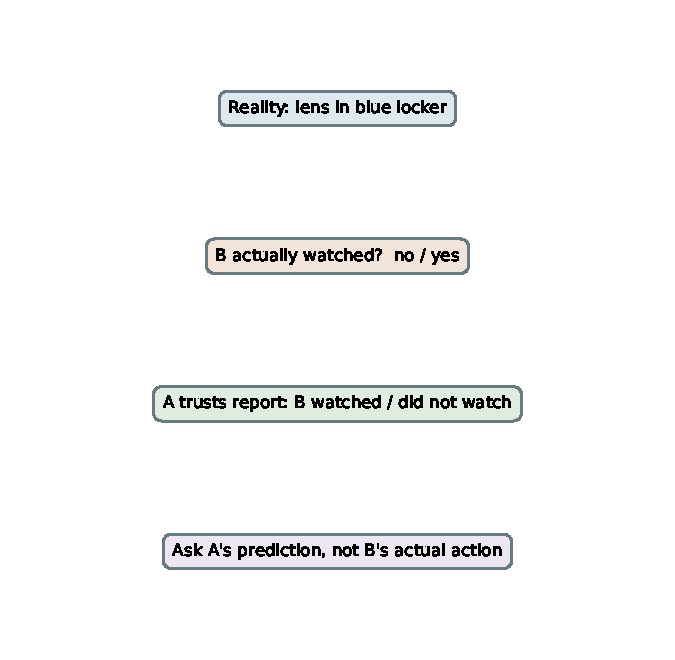
\includegraphics[width=\linewidth]{02/results/belief_intervention.pdf}
\caption{二次信念の対照設計。相手の実際の情報と、予測者が信用する報告を分離する。質問は相手の実行動ではなく予測者による予測を求める。}
\end{figure}

皮肉では、同じ肯定表現に対して仕事の失敗と成功という文脈を変えた。
失言では、作者の目の前で作品を批判した発言者について、作者を知らなかった場合と知っていた場合を区別した。
どちらも相手は傷つきうるので、「失礼かどうか」と「作者を知らないことによる失言かどうか」を同一視しない。
情報不足群では、褒め言葉しか残っていないメッセージから、皮肉か称賛かを確定できるかを問う。

\subsection{回答取得と採点}
作成後のv2プロンプトJSONを固定し、親会話を引き継がない二つの新規コンテキストのCodexサブエージェントへ渡した。
各回答者が読めるファイルを上記の刺激JSON一つに限定し、正解・群分け・生成コード・旧版データ・相互の回答を見せず、選択肢と短い根拠を保存した。
モデルは\texttt{gpt-6.1-sol}、実施日は2026年11月17日である。
温度など内部の生成設定は取得できない。
各コンテキストには44項目を一括提示しており、項目ごとに独立した44会話を作ったわけではない。
問題と条件には共有構造もあるため、88件を独立した標本として検定しない。
元データ、生回答、正解、採点コード、刺激のSHA-256ハッシュを保存し、取得後に監査できる構成とした。

\subsection{修正版の実測結果と対照}
両コンテキストとも44/44項目を正答し、20/20組の最小対に成功した。
コンテキスト間の選択肢一致も44/44であった。
二次信念で実際の知識と予測者の信念が食い違う8項目も、両コンテキストとも8/8正答した。
常にA、B、Cを選ぶ対照はそれぞれ14/44、14/44、16/44であった。
信念2群で常に物の最終場所を答える対照は12/24、二次信念群で相手の実際の知識だけから答える対照は8/16である。

\begin{table}[tb]\centering\footnotesize
\caption{v2の群別正答数。最小対は両問正答で1組とする。44項目の全文と個別の短い根拠は公開JSONに保存。}
\begin{tabular}{lrrr}\toprule
項目群 & 項目数 & 文脈1 & 文脈2\\\midrule
一次信念 & 8 & 8 & 8\\
二次信念 & 16 & 16 & 16\\
皮肉 & 8 & 8 & 8\\
失言の知識 & 8 & 8 & 8\\
情報不足 & 4 & 4 & 4\\
\midrule
最小対の両問正解 & 20組 & 20 & 20\\
\bottomrule\end{tabular}

\end{table}

\begin{figure}[tb]\centering
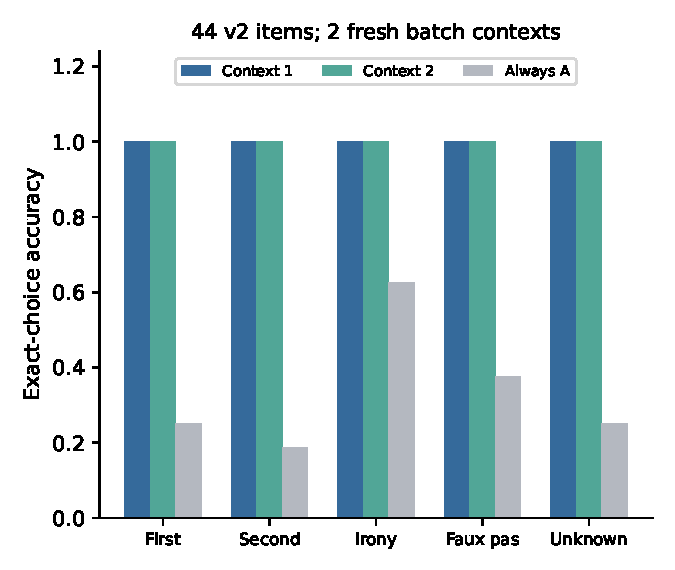
\includegraphics[width=\linewidth]{02/results/accuracy.pdf}
\caption{二つの新規コンテキストと固定回答対照の正答率。二次信念は16項目、一次・皮肉・失言は各8項目、情報不足は4項目。}
\end{figure}

例えば、実際には航が映像を見ていないが綾が見たと信じる項目で、文脈1は「綾は航が映像を見たという報告を信じているため、実際の故障にかかわらず青いロッカーを探すと予測する。」と説明した。
反対方向の不一致にも対応し、岳が澪は見ていないと信じる場合は、澪が実際に見ていても元の棚を選んだ。
情報不足群では、両コンテキストとも称賛か皮肉かを無理に確定しなかった。
これらは、今回の明示的で短い日本語物語では、現実・相手の情報・予測者の信念を区別した答えを生成できたという観察である。
一方、全問正解という天井効果のため、能力の上限や誤りやすい境界は特定できなかった。
信頼する報告の文言を対応づける規則でも解ける構成なので、柔軟なToMの獲得まで結論を広げない。

\subsection{ヒトとの類似性・相違と今後のデータ}
ヒトとの類似性は、観察していない出来事を他者が知らないと扱い、同じ言葉を状況に応じて解釈し、情報不足を認めるという出力の特徴にある。
一方、人間は視線・声の調子・身体の動き・過去の対人関係からも判断する。
今回のLLMは、情報アクセスや報告への信用を実験者が明示した文章から解いた。
人間の対照群を測定していないため、100\%という結果から人間以上と結論づけることはできない。
出題にも同系列のLLMを利用しており、出題側と回答側の独立性にも限界がある。
また、識別子と表示順の監査で既知の抜け道は除いたが、あらゆる表面的な解法を排除できたとは主張しない。

類推推論では、レンズ・センサー・鍵・基板といった対象の置換だけでなく、「他者が接した情報によって信念を更新する」という関係を別の課題に対応させられるかが焦点になる。
例えばソフトウェアのアクセス権、共同作業の共有履歴、誤った地図を使う相手との協調へ移すテストが考えられる。
この種の類推は強いAIの研究に有用な仮説だが、その十分条件が証明されたわけではない。

今後集めるべきデータは、各人物が各時点で何を見聞きしたかを注釈した時系列対話、情報を隠す協調課題、誤解を指摘した後に信念を修正する長期的対話である。
正解ラベルに加えて、情報不足による不確実性、文化や関係性の違いで複数解が妥当になる範囲も記録したい。
評価では作成者とモデル系列を分け、未公開項目を独立に作り、文順・言い換え・不要情報・暗黙の観察機会への頑健性を調べる必要がある。
公開後に同じ項目で将来モデルを測る場合には、学習データへの混入も考慮すべきである\cite{tomreview}。
\repolink{02}
